\documentclass[11pt]{article}

\usepackage[margin=1in]{geometry}
\usepackage[T1]{fontenc}
\usepackage[utf8]{inputenc}
\usepackage{lmodern}
\usepackage{microtype}
\usepackage{setspace}
\usepackage{graphicx}
\usepackage{booktabs}
\usepackage{caption}
\usepackage{array}
\usepackage{amsmath,amssymb}
\usepackage[hidelinks,hypertexnames=false]{hyperref}
\usepackage[nameinlink,noabbrev]{cleveref}
\usepackage{float}
\graphicspath{{figures/}}

\onehalfspacing
\setlength{\parskip}{0.5em}
\setlength{\parindent}{0pt}
\setlength{\textfloatsep}{8pt plus 1pt minus 2pt}
\setlength{\floatsep}{6pt plus 1pt minus 2pt}
\setlength{\intextsep}{6pt plus 1pt minus 2pt}
\captionsetup{skip=4pt}

\title{Supplementary Material for\\Score-Aware Expert Combination for Protocol-Aware Multimodal Knowledge Graph Completion under Incomplete Visual Support}
\author{}
\date{}

\begin{document}

\maketitle

\appendix

\section{Clean Routing Progression and Hard-selection Oracle Headroom}
\label{app:clean_oracle_gap}

\begin{figure}[H]
    \centering
    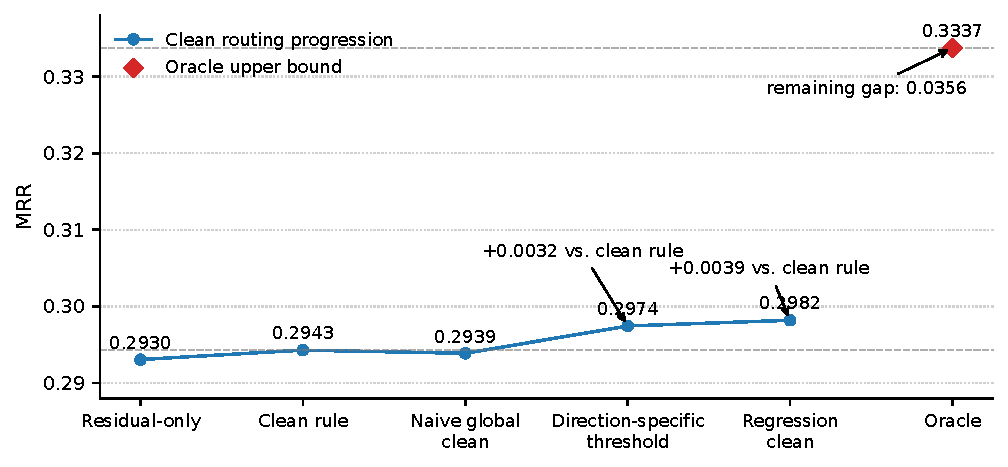
\includegraphics[width=0.86\textwidth]{figures/Figure_clean_vs_oracle_gap.pdf}
    \caption{MRR progression from fixed structural fallback to stronger clean routing and hard-selection Oracle routing on the clean evaluation line.}
    \label{fig:clean_vs_oracle_gap}
\end{figure}

\section{Additional Delta Sensitivity Results}
\label{app:delta_sensitivity}

\begin{table}[H]
\centering
\caption{Delta sensitivity of naive global-threshold clean routing.}
\label{tab:delta_sensitivity}
\small
\begin{tabular}{lccc}
\toprule
Model & $\delta$ & Best $\tau$ & Best MRR \\
\midrule
Logistic & 0.00 & 0.5 & 0.2978 \\
Logistic & 0.01 & 0.9 & 0.2939 \\
Logistic & 0.02 & 0.9 & 0.2935 \\
XGBoost & 0.00 & 0.5 & 0.2983 \\
XGBoost & 0.01 & 0.9 & 0.2939 \\
XGBoost & 0.02 & 0.9 & 0.2938 \\
\bottomrule
\end{tabular}
\end{table}

\section{Candidate-level Router Diagnostics}
\label{app:candidate_router_diagnostics}

\begin{table}[H]
\centering
\small
\caption{Candidate-aware full-ranking results by target-side regime.}
\label{tab:candidate_router_subgroup_results}
\resizebox{\textwidth}{!}{%
\begin{tabular}{p{0.18\textwidth}p{0.14\textwidth}ccccc}
\toprule
Method & Regime & \#Queries & Gate MRR & Residual MRR & Method MRR & Delta vs Residual \\
\midrule
CA-S1 clean candidate & head\_has\_img & 7048 & 0.0134 & 0.0017 $\pm$ 0.0001 & 0.0052 $\pm$ 0.0004 & +0.0034 $\pm$ 0.0003 \\
CA-S1 clean candidate & head\_no\_img & 2952 & 0.0123 & 0.0055 $\pm$ 0.0003 & 0.0180 $\pm$ 0.0013 & +0.0125 $\pm$ 0.0015 \\
CA-S1 clean candidate & tail\_no\_img & 10000 & 0.3945 & 0.5832 $\pm$ 0.0015 & 0.4917 $\pm$ 0.0103 & -0.0916 $\pm$ 0.0116 \\
CA-S2 score-aware & head\_has\_img & 7048 & 0.0134 & 0.0017 $\pm$ 0.0001 & 0.0032 $\pm$ 0.0002 & +0.0015 $\pm$ 0.0001 \\
CA-S2 score-aware & head\_no\_img & 2952 & 0.0123 & 0.0055 $\pm$ 0.0003 & 0.0081 $\pm$ 0.0004 & +0.0026 $\pm$ 0.0003 \\
CA-S2 score-aware & tail\_no\_img & 10000 & 0.3945 & 0.5832 $\pm$ 0.0015 & 0.6236 $\pm$ 0.0019 & +0.0404 $\pm$ 0.0025 \\
CA-S3 clean + score & head\_has\_img & 7048 & 0.0134 & 0.0017 $\pm$ 0.0001 & 0.0034 $\pm$ 0.0002 & +0.0017 $\pm$ 0.0001 \\
CA-S3 clean + score & head\_no\_img & 2952 & 0.0123 & 0.0055 $\pm$ 0.0003 & 0.0079 $\pm$ 0.0007 & +0.0024 $\pm$ 0.0004 \\
CA-S3 clean + score & tail\_no\_img & 10000 & 0.3945 & 0.5832 $\pm$ 0.0015 & 0.6222 $\pm$ 0.0016 & +0.0389 $\pm$ 0.0013 \\
\bottomrule
\end{tabular}
}
\vspace{0.4ex}\caption*{\footnotesize The overall gain is primarily driven by the tail-side regime, while head-side gains remain small in absolute MRR.}
\end{table}

\begin{table}[H]
\centering
\small
\caption{Overall alpha behavior of candidate-aware full-ranking routers.}
\label{tab:candidate_router_alpha_overall}
\begin{tabular}{p{0.22\textwidth}cccc}
\toprule
Method & Mean alpha & Target alpha & Target/mean alpha & MRR gain vs Residual \\
\midrule
CA-S1 clean candidate & 0.3811 $\pm$ 0.0000 & 0.2570 $\pm$ 0.0000 & 0.6744 & -0.0427 $\pm$ 0.0061 \\
CA-S2 score-aware & 0.0470 $\pm$ 0.0001 & 0.1964 $\pm$ 0.0084 & 4.1768 & +0.0211 $\pm$ 0.0012 \\
CA-S3 clean + score & 0.0480 $\pm$ 0.0004 & 0.2016 $\pm$ 0.0085 & 4.1997 & +0.0204 $\pm$ 0.0007 \\
\bottomrule
\end{tabular}
\vspace{0.4ex}\caption*{\footnotesize The target/mean alpha ratio summarizes how selectively the router raises fusion weight on the correct entity.}
\end{table}

The omitted regime-level alpha table follows the same qualitative pattern as the subgroup MRR table: score-aware routers remain mostly structural over the candidate set while assigning larger fusion weight to target candidates, especially in the dominant \texttt{tail\_no\_img} regime.

\clearpage
\section{Additional Protocol Sanity Checks}
\label{app:protocol_sanity}

Relation-group evidence provides a supporting view of the bounded-gain structure. Only relations with at least 20 test queries are retained.

\begin{table}[H]
\centering
\caption{Relation-type grouped MRR under the unified OpenBG-IMG protocol.}
\label{tab:relation_grouped}
\small
\setlength{\tabcolsep}{5pt}
\begin{tabular}{lccc}
\toprule
Model & \texttt{visual\_relations} & \texttt{weak\_visual\_relations} & \texttt{ambiguous\_material\_relations} \\
\midrule
\texttt{Residual-only} & 0.2691 $\pm$ 0.0011 & 0.3197 $\pm$ 0.0010 & 0.2842 $\pm$ 0.0028 \\
\texttt{Full Model} & 0.1826 $\pm$ 0.0071 & 0.2252 $\pm$ 0.0154 & 0.1948 $\pm$ 0.0201 \\
\texttt{Gate-only} & 0.1350 $\pm$ 0.0068 & 0.2194 $\pm$ 0.0073 & 0.1337 $\pm$ 0.0083 \\
\bottomrule
\end{tabular}
\end{table}

\begin{table}[H]
\centering
\caption{Retained support for relation-group analysis after minimum-support filtering.}
\label{tab:relation_group_support}
\small
\begin{tabular}{lcc}
\toprule
Group & \#Relations retained & \#Test queries retained \\
\midrule
\texttt{visual\_relations} & 24 & 3{,}804 \\
\texttt{weak\_visual\_relations} & 18 & 3{,}304 \\
\texttt{ambiguous\_material\_relations} & 9 & 1{,}150 \\
\bottomrule
\end{tabular}
\end{table}

We add a lightweight degree-based sanity check to examine whether the target-side role--modality pattern is reducible to an unexamined degree artifact. Entity degree is computed only from the training graph, using the number of train triples in which an entity appears as head or tail. The results are reported by test-time target-side regime.

\begin{table}[t]
\centering
\small
\caption{Training-graph degree by test-time target-side regime. Entity degree is computed only from training triples.}
\label{tab:degree_by_target_regime}
\begin{tabular}{lrrrrrr}
\toprule
Regime & \#Queries & Mean degree & Median degree & Q25 & Q75 & Mean log-degree \\
\midrule
\texttt{head\_has\_img} & 7,048 & 10.86 & 11.00 & 8.00 & 13.00 & 2.42 \\
\texttt{head\_no\_img} & 2,952 & 11.54 & 11.00 & 8.00 & 14.00 & 2.42 \\
\texttt{tail\_no\_img} & 10,000 & 3169.69 & 1517.00 & 274.00 & 3368.00 & 6.82 \\
\bottomrule
\end{tabular}
\end{table}


The table shows that the dominant \texttt{tail\_no\_img} regime is also much higher-degree than the two head-side regimes under the training graph. This analysis therefore does not remove structural confounding from the benchmark, and it should not be read as proving that modality availability alone explains the observed asymmetry. Instead, it makes the main interpretation more explicitly protocol-aware: degree and modality availability may both contribute to the bounded-gain structure, while the routing experiments directly test how much deployable gain can be recovered under this protocol.

\end{document}
